% ==============================================================================
% SEZIONE 2 — APPLICAZIONI BIOMEDICALI DELLE SNN IN SISTEMI IMPIANTABILI
% ==============================================================================
\section[Applicazioni biomedicali impiantabili]{Applicazioni biomedicali delle SNN nei sistemi impiantabili}
\label{sec:applicazioni}

\subsection{Vincoli dei dispositivi impiantabili e ruolo della codifica a spike}
\label{subsec:vincoli_impiantabili}


Progettare un dispositivo elettronico impiantabile è molto più complicato rispetto a un normale dispositivo indossabile, perché ci sono diversi vincoli fisici da rispettare. 

Il primo riguarda il calore generato dal chip. Lavorando a contatto con il tessuto cerebrale, la potenza dissipata deve rimanere bassissima per non surriscaldare il tessuto stesso. Come riferimento, un singolo neurone biologico consuma per la sua attività metabolica circa $0{,}5\text{--}\SI{4{,}0}{\nano\watt}$, una quantità di calore che il nostro corpo riesce a smaltire normalmente~\cite{ronchini2023}. 

A questo si aggiungono i limiti di spazio e di consumo energetico. Nei dispositivi impiantabili è fondamentale tenere bassi sia l'area occupata sia la potenza assorbita, in modo da avere sistemi compatti e far durare il più possibile la batteria~\cite{ronchini2023, wu2026}. Il problema diventa ancora più evidente nelle interfacce neurali moderne, che possono arrivare fino a migliaia di canali di registrazione~\cite{wu2026}: acquisire di continuo tutti questi segnali e inviarli via wireless verso l'esterno consumerebbe troppa energia. Per questo conviene elaborare i segnali direttamente sul chip, riducendo la quantità di dati da trasmettere~\cite{ronchini2023, wu2026}.

Un ultimo vincolo importante riguarda i tempi di risposta, ovvero la latenza. Un esempio concreto è la stimolazione cerebrale profonda (DBS), usata per trattare l'epilessia nei pazienti che non rispondono ai farmaci, circa il 30\% dei casi~\cite{ronchini2023}. Questo tipo di stimolazione può funzionare in due modi, open loop o closed loop. Nei sistemi open loop non c'è alcuna retroazione, quindi il dispositivo invia impulsi elettrici in modo continuo secondo uno schema fisso, senza tenere conto di cosa sta succedendo nel cervello; invece nei sistemi closed loop il dispositivo registra l'attività cerebrale, la analizza e invia lo stimolo elettrico solo quando riconosce i segnali tipici di una crisi~\cite{ronchini2023}. L'approccio closed loop risulta più efficace e ha meno effetti collaterali, perchè interviene solo quando serve, ma per riuscire a intervenire in tempo il dispositivo deve riconoscere la crisi localmente e con una latenza molto bassa, nell'ordine dei millisecondi~\cite{ronchini2023}.

Il primo passo comune a tutte le applicazioni biomedicali basate su SNN è convertire il segnale biologico in una sequenza di spike. Tutti i paper che ho analizzato hanno la stessa idea di fondo: generano uno spike solo quando il segnale sale o scende superando una certa soglia. Ecco come avviene nel dettaglio nei paper:
\begin{itemize}
  \item Step-Forward Encoding (SFE), usato in NET-TEN~\cite{ronchini2023}: lavora sui segnali LFP (cioè i potenziali di campo locale), che sono segnali elettrici registrati direttamente nel tessuto cerebrale. L'algoritmo prende il primo valore del segnale come livello di riferimento (chiamato baseline nel paper) e fissa una soglia, definendo una fascia tra $\text{baseline} - \text{soglia}$ e $\text{baseline} + \text{soglia}$. Per quanto riguarda i campioni successivi, se il segnale esce verso l'alto viene generato uno spike di salita e la baseline sale del valore della soglia; se scende sotto la fascia viene generato uno spike di discesa e la baseline scende della stessa quantità. Finché il segnale resta dentro questa fascia non viene emesso nessuno spike.
  \item Asynchronous Delta Modulation (ADM), integrato sul chip DYNAP-SE2~\cite{bartels2025}: a differenza di SFE (che è eseguito via software), qui generazione di spike avviene tramite un circuito analogico posto subito dopo l'amplificatore del segnale EEG intracranico. Ogni volta che l'ampiezza varia di più di una soglia prefissata, genera uno spike di salita se il segnale sta crescendo, oppure di discesa se sta diminuendo. In questo modo produce molti spike solo quando il segnale varia rapidamente, come durante una crisi, e quasi nessuno nei momenti di quiete.
  \item Analog-to-Spike Converter (ASC), usato in NeuroSEED~\cite{wu2026}: anche in questo caso la generazione avviene in hardware. Due comparatori controllano continuamente se il segnale supera una soglia superiore o scende sotto una soglia inferiore: appena succede, il circuito emette uno spike di salita o di discesa, e tramite un piccolo DAC capacitivo da 1 bit, riporta subito la tensione al livello intermedio di riferimento (così da poter rilevare la variazione successiva senza andare in saturazione). C'è poi un blocco refrattario che aggiunge una breve pausa dopo ogni spike per limitare la frequenza massima di uscita.
  \item Codifica Delta-Sigma, usata con Xylo~\cite{li2024}: viene applicata via software al segnale EEG di scalpo già filtrato. Divide l'escursione di ampiezza del segnale in livelli fissi equidistanti. Ogni volta che il segnale attraversa uno di questi livelli, viene generato uno spike di salita se sta crescendo oppure uno spike di discesa se sta diminuendo. Durante una crisi epilettica, dato che il segnale EEG diventa più ampio e oscilla più velocemente, attraversa molti più livelli e produce quindi una sequenza di spike molto più fitta.
\end{itemize}


\subsection{Rilevamento di eventi epilettici da LFP: NET-TEN (Ronchini et al., 2023)}
\label{subsec:netten_app}

Il chip NET-TEN, presentato da Ronchini et al.\ (2023)~\cite{ronchini2023}, è un esempio di rete neuromorfica pensata per un dispositivo impiantabile. È realizzato interamente con circuiti analogici in tecnologia CMOS \SI{180}{\nano\meter} fatti lavorare in sottosoglia, occupa un'area di \SI{1{,}08}{\milli\meter\squared} ed è alimentato a soli $\Vdd = \SI{250}{\milli\volt}$. Il suo scopo è riconoscere gli eventi epilettici a partire dai potenziali di campo locale (LFP). Rileva sia le crisi vere e proprie (eventi ictali), sia le scariche brevi che possono comparire tra una crisi e l'altra (eventi interictali)~\cite{ronchini2023}.

Per testare il chip, gli autori hanno usato segnali registrati in vitro da 10 fettine di cervello di topo, prese da 10 animali diversi così da includere la variabilità biologica. Le fettine sono state trattate con una sostanza chimica (la 4-aminopiridina, 4AP) che induce attività epilettica, e poi appoggiate su una matrice di elettrodi (MEA $6\times 10$) campionando il segnale LFP a \SI{2}{\kilo\hertz}. Da queste registrazioni sono stati estratti 10 segmenti da \SI{100}{\second}: 9 contengono una crisi ictale (di cui 3 includono anche scariche interictali), mentre uno contiene soltanto un artefatto elettrico, cioè un disturbo non dovuto a una crisi~\cite{ronchini2023}.

Prima di arrivare al chip, questi segnali LFP vengono convertiti in spike via software (in MATLAB) con l'algoritmo SFE visto sopra. Dato che una soglia più bassa genera più spike e una più alta ne genera meno, la soglia viene regolata in modo che circa il 30\% dei campioni totali produca uno spike. Le sequenze digitali così ottenute vengono poi trasformate in impulsi elettrici e inviate ai 10 neuroni d'ingresso di NET-TEN. Cinque ricevono gli spike di salita e gli altri cinque quelli di discesa~\cite{ronchini2023}.


La rete è fatta da 3 strati in cascata, formati da 10 neuroni ciascuno, basati sul modello di Izhikevich. Ogni neurone d'ingresso si collega a due neuroni dello strato intermedio, mentre tra lo strato intermedio e quello di uscita le connessioni sono uno a uno. Ogni collegamento utilizza una sinapsi eccitatoria (EPSC) abbinata a un circuito di plasticità STDP, che regola il peso della sinapsi in base alla distanza temporale tra gli spike dei due neuroni collegati. Anche se tutti i circuiti condividono le stesse tensioni di polarizzazione, dato che stiamo lavorando in sottosoglia, il mismatch comporta che i neuroni non si comportino tutti esattamente allo stesso modo. Misurando tutte e 10 le uscite del chip, solo 4 canali hanno prodotto risultati utili~\cite{ronchini2023}.

I risultati ottenuti su questi 4 canali sono mostrati in figura~\ref{fig:netten_app}. Prima di tutto i consumi sono bassissimi: la potenza statica è di appena \SI{0{,}68}{\pico\watt}, mentre la potenza media durante il rilevamento è di \SI{3{,}50}{\nano\watt}. Come visto prima, si tratta di un valore paragonabile al consumo metabolico di un singolo neurone biologico ($0{,}5\text{--}\SI{4{,}0}{\nano\watt}$), quindi il calore prodotto non rischierebbe di danneggiare il tessuto cerebrale. Inoltre si raggiunge una precisione di 0,998 (quasi nessun falso allarme) e risponde con un ritardo medio di \SI{110{,}4}{\milli\second} per una crisi ictale e di \SI{126{,}6}{\milli\second} per una interictale ~\cite{ronchini2023}.


Gli autori hanno poi provato a capire come distinguere tra crisi ictale, scarica interictale e un semplice artefatto elettrico, e hanno notato che: quando inizia una crisi o una scarica, gli spike iniziali arrivano molto ravvicinati tra loro, mentre con l'artefatto sono molto più distanziati; una crisi ictale produce moltissimi spike (mediana di 1117,5), contro pochissimi per una scarica interictale (mediana di 4,5) e un valore intermedio per l'artefatto (mediana di 27,5). Propongono questa regola: prima si verifica che tra il primo e il terzo spike passino meno di \SI{10}{\milli\second} (scartando così l'artefatto), poi si controlla che nei successivi \SI{190}{\milli\second} arrivino almeno altri 10 spike (distinguendo la crisi vera e propria da una scarica interictale). Questa logica può essere integrata sul chip con due semplici contatori digitali (un contatore temporale che aggiunge appena \SI{31}{\pico\watt} e un piccolo contatore di spike dal consumo trascurabile). La potenza totale è praticamente rimasta invariata, e comunque il ritardo di riconoscimento resta sotto lo 0,6\% della durata mediana di una crisi~\cite{ronchini2023}.

\begin{figure}[tb]
  \centering
  \begin{subfigure}[b]{0.53\textwidth}
    \centering
    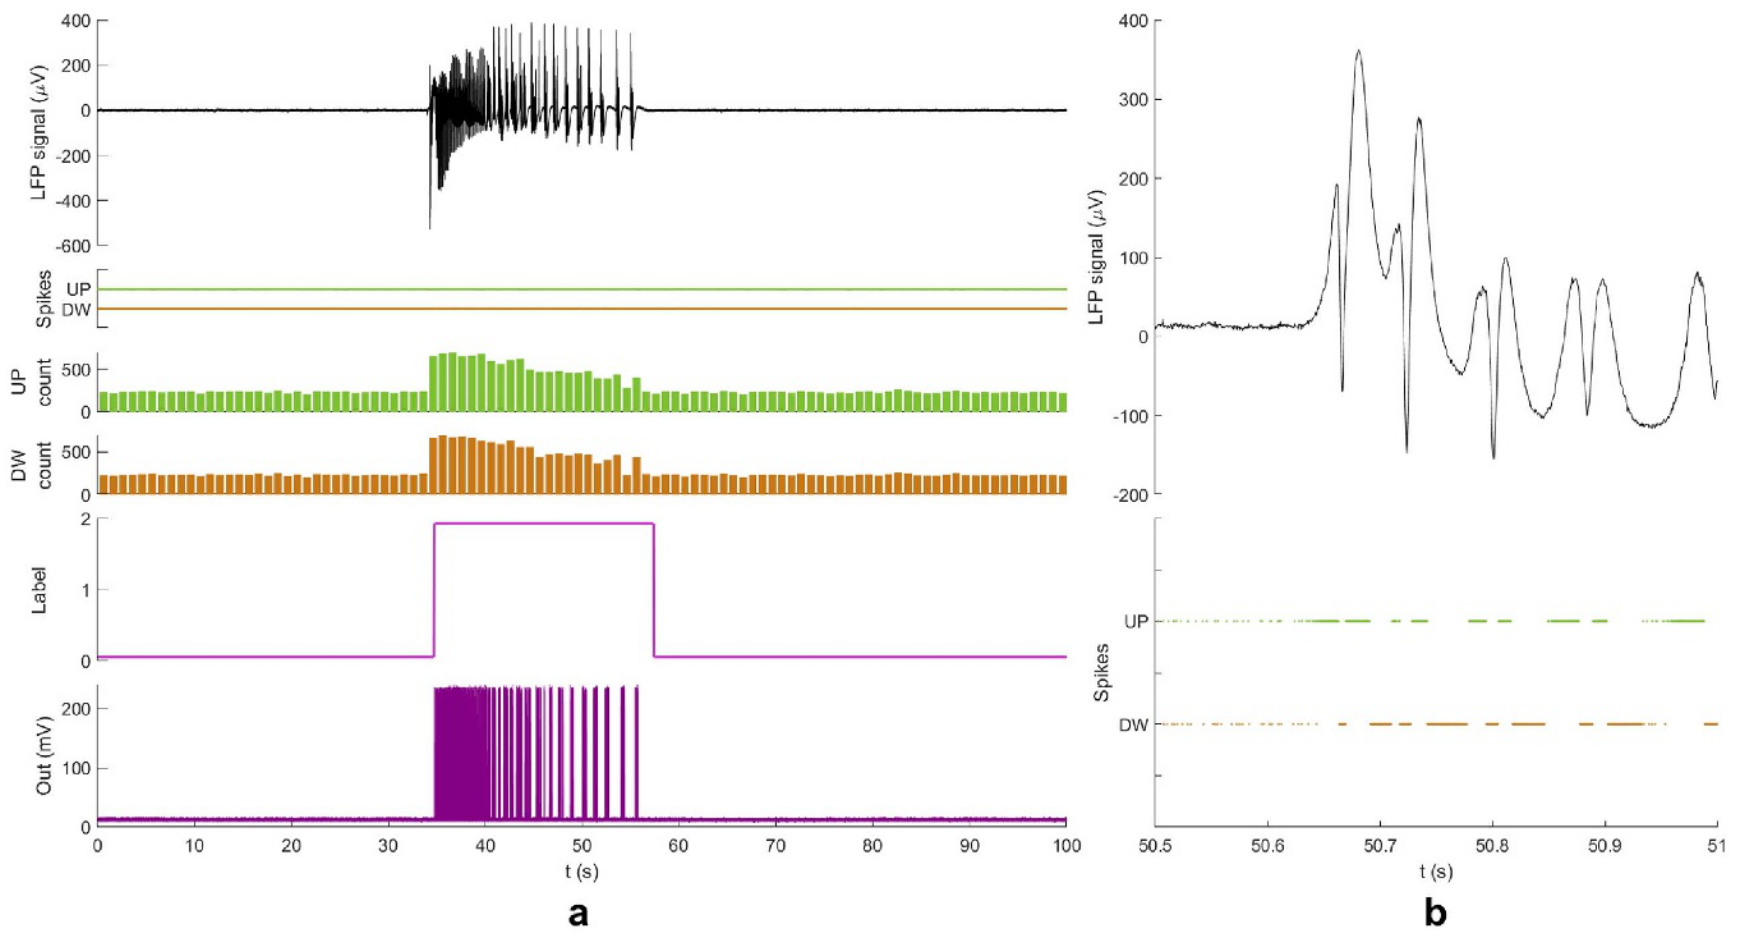
\includegraphics[width=\linewidth]{netten_lfp_detection.png}
    \caption{}
  \end{subfigure}
  \hfill
  \begin{subfigure}[b]{0.45\textwidth}
    \centering
    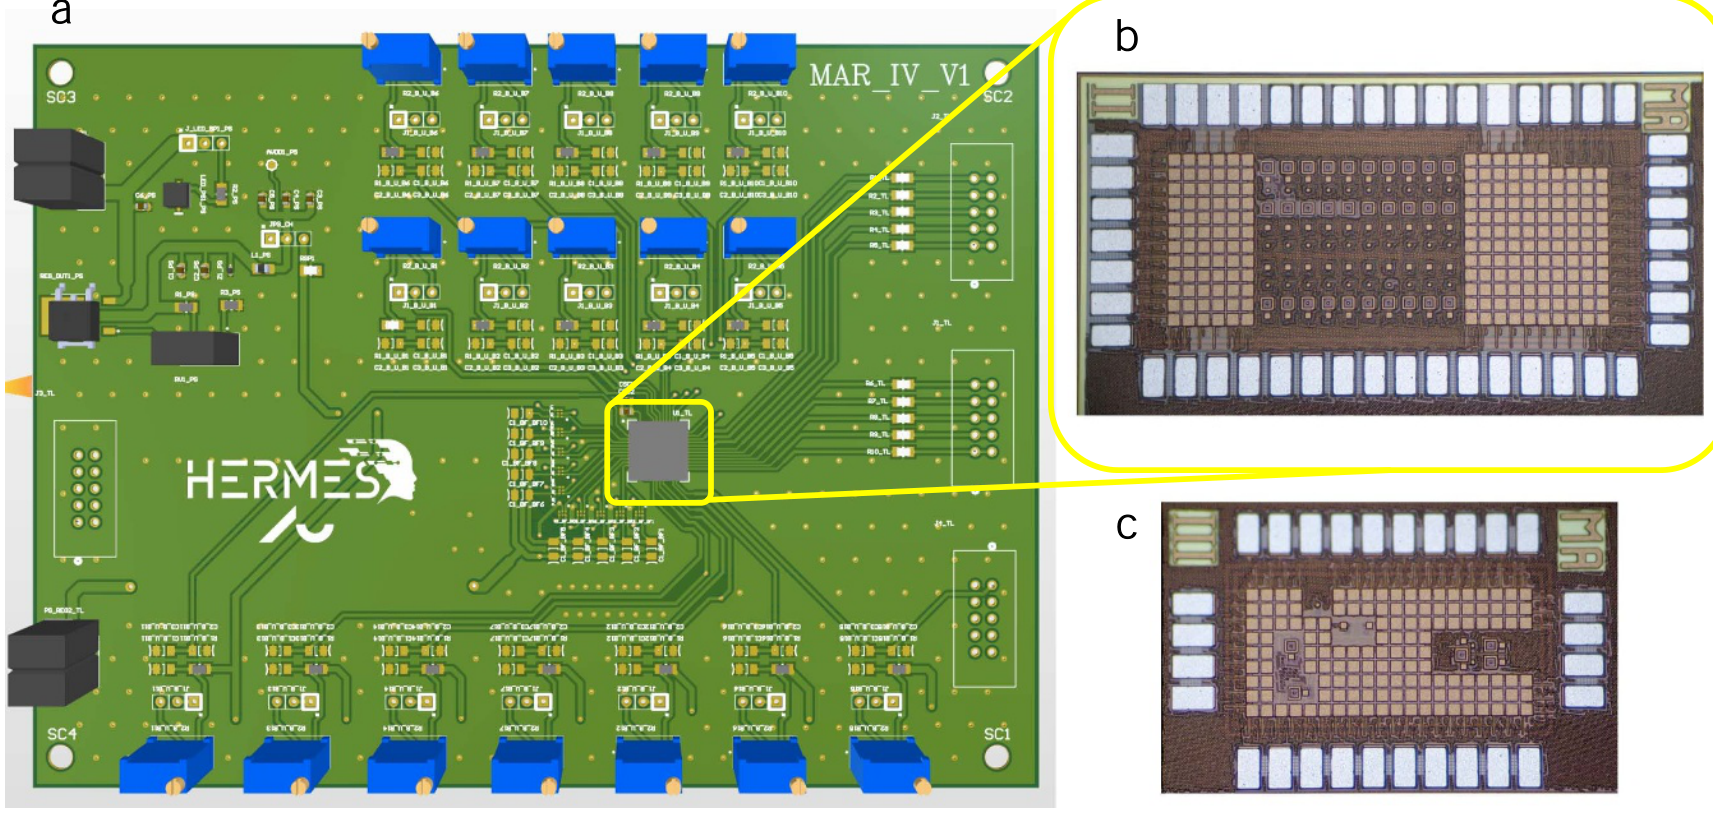
\includegraphics[width=\linewidth]{netten_pcb_die.png}
    \caption{}
  \end{subfigure}
  \caption[Sistema NET-TEN: rilevamento ictale da LFP e die CMOS]{(a) Esempio di tracciato LFP di \SI{100}{\second} di una crisi ictale; (b) PCB usata per la caratterizzazione, con die NET-TEN ~\cite{ronchini2023}}
  \label{fig:netten_app}
\end{figure}

Nel paper vengono tuttavia mostrati i limiti di questo prototipo: l'acquizione, il filtraggio e la codifica SFE avvengono via software, fuori dal chip; le tensioni di bias sono regolate manualmente tramite potenziometri, e i condensatori STDP utilizzati trattengono i pesi solo per tempi nell'ordine di decine di millisecondi, quindi non c'è apprendimento permanente~\cite{ronchini2023}.

\subsection{Un sistema impiantabile completo: NeuroSEED (Wu et al., 2026)}
\label{subsec:neuroseed_app}

Nel paper di Wu et al.\ (2026)~\cite{wu2026} si affronta il problema di realizzare un sistema neurale impiantabile completo su un singolo chip. Il sistema si chiama NeuroSEED: è realizzato in tecnologia CMOS \SI{40}{\nano\meter}, è alimentato a \SI{1{,}2}{\volt} e occupa un'area totale di \SI{0{,}70}{\milli\meter\squared}. Gestisce 32 canali per rilevare i potenziali d'azione (in banda fino a \SI{5{,}2}{\kilo\hertz}) e trasmetterli via wireless verso l'esterno. NeuroSEED è organizzato in quattro blocchi principali, mostrati in figura~\ref{fig:neuroseed_arch}.

Il primo blocco è lo stadio di acquisizione analogico di 32 canali. Il chip usa un solo amplificatore a basso rumore condiviso tra i 32 elettrodi tramite una serie di interruttori che leggono i canali a turno (tecnica chiamata multiplexing nel tempo, TDM). Ogni canale viene così campionato a \SI{10{,}4}{\kilo\hertz}, una frequenza sufficiente per rilevare i potenziali d'azione senza sprecare energia con frequenze più alte. Condividere l'amplificatore riduce drasticamente l'area di ingresso a soli \SI{0{,}0032}{\milli\meter\squared} per canale, mantenendo un rumore molto basso (\SI{2{,}9}{\micro\volt\textsubscript{rms}}) e un guadagno regolabile tra \SI{41{,}2}{\decibel} e \SI{58{,}3}{\decibel} per compensare le variazioni dell'impedenza degli elettrodi nel tempo~\cite{wu2026}.

Il secondo blocco serve a cancellare l'offset DC che si crea all'interfaccia tra elettrodo e tessuto biologico, che può arrivare fino a $\pm\SI{50}{\milli\volt}$. C'è un anello di controllo digitale che ogni \SI{4{,}8}{\second} esegue una calibrazione da \SI{0{,}96}{\milli\second}. Misura l'offset medio sfruttando gli spike del convertitore ASC (descritto nella Sezione~\ref{subsec:vincoli_impiantabili}), lo accumula in un contatore a 6 bit e applica all'ingresso una tensione uguale e opposta tramite un DAC capacitivo a 6 bit~\cite{wu2026}.

Il terzo blocco riguarda la conversione in spike e il riconoscimento dei potenziali d'azione. Dopo la parte di amplificazione, il segnale viene di nuovo separato nei 32 canali, ciascuno dotato del convertitore ASC e di un piccolo rivelatore asincrono senza clock, che quindi consuma solo quando arrivano eventi. Il rivelatore capisce qual'è il minimo del segnale e da lì conta quanti spike di salita arrivano fino al picco successivo. Questo conteggio misura di quanto si è alzato il segnale dal punto più basso al punto più alto, e se la salita supera una soglia programmabile, il circuito riconosce un potenziale d'azione vero e proprio, filtrando così le oscillazioni del rumore di fondo. Questo blocco occupa \SI{0{,}0007}{\milli\meter\squared} e consuma \SI{0{,}48}{\micro\watt} per canale~\cite{wu2026}.

L'ultimo blocco è il trasmettitore wireless. Il fatto di riconoscere i potenziali d'azione direttamente sul chip riduce notevolmente il volume di dati da inviare all'esterno. Il trasmettitore integrato (IR-UWB, a \SI{4{,}25}{\giga\hertz}) si accende solo quando viene riconosciuto un potenziale d'azione. In questo modo il suo consumo medio scende a \SI{4{,}6}{\micro\watt} totali~\cite{wu2026}.

% --- FIGURA 2.3: Diagramma a blocchi NeuroSEED (da Wu et al., 2026) ---
\begin{figure}[tb]
  \centering
  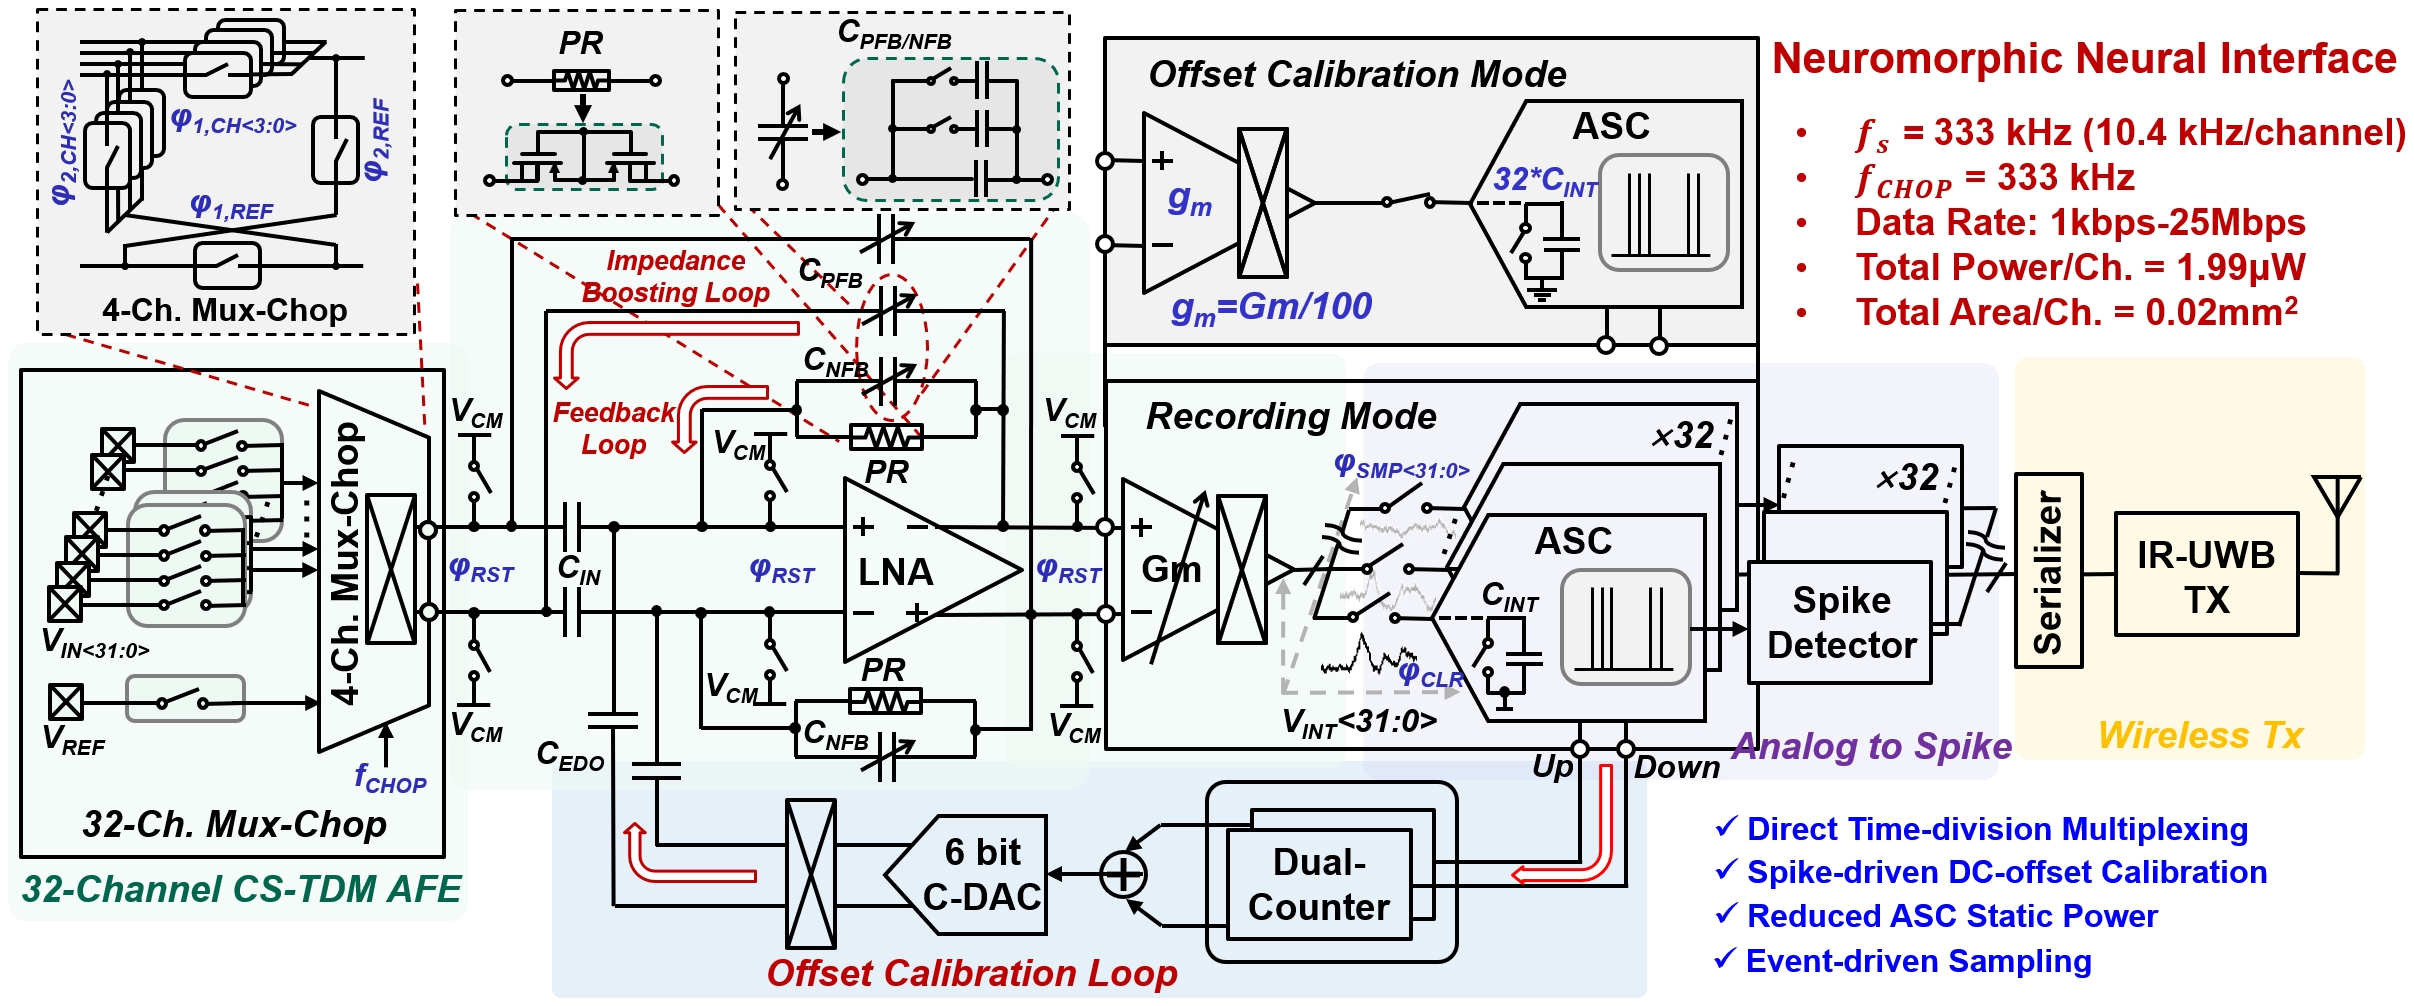
\includegraphics[width=\textwidth]{neuroseed_arch.png}
  \caption[Architettura del chip NeuroSEED]{Architettura del chip NeuroSEED~\cite{wu2026}.}
  \label{fig:neuroseed_arch}
\end{figure}

Il chip, mostrato in figura~\ref{fig:neuroseed_silicio}a, consuma nel complesso \SI{63{,}61}{\micro\watt}, pari a \SI{1{,}99}{\micro\watt} per canale. Come si vede in figura~\ref{fig:neuroseed_silicio}b, è stato testato su dei dati registrati in vivo su ratto e riesce a tracciare in modo affidabile i potenziali d'azione riducendo drasticamente i dati da trasmettere~\cite{wu2026}.

\begin{figure}[tb]
  \centering
  \begin{subfigure}[b]{0.52\textwidth}
    \centering
    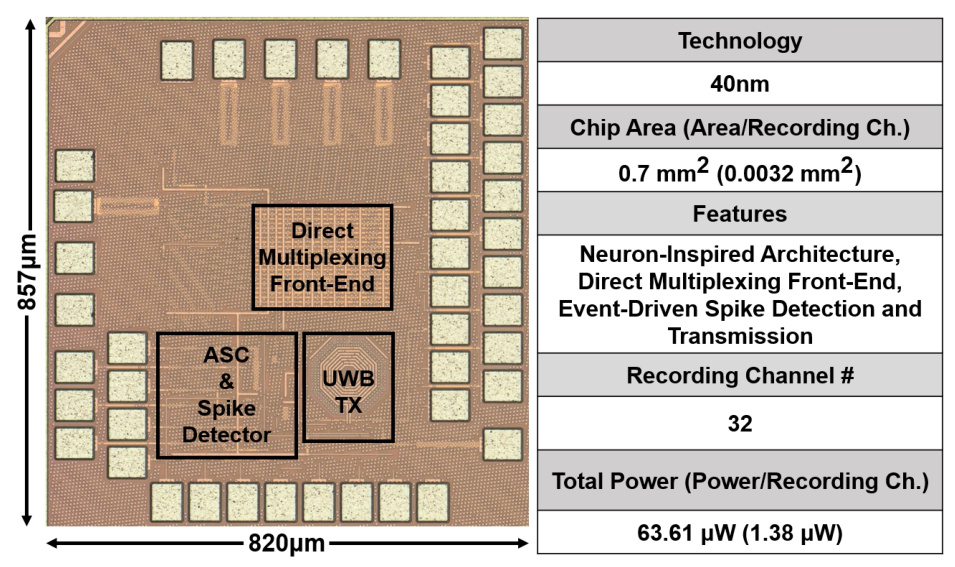
\includegraphics[width=\linewidth]{neuroseed_die.png}
    \caption{}
  \end{subfigure}
  \hfill
  \begin{subfigure}[b]{0.44\textwidth}
    \centering
    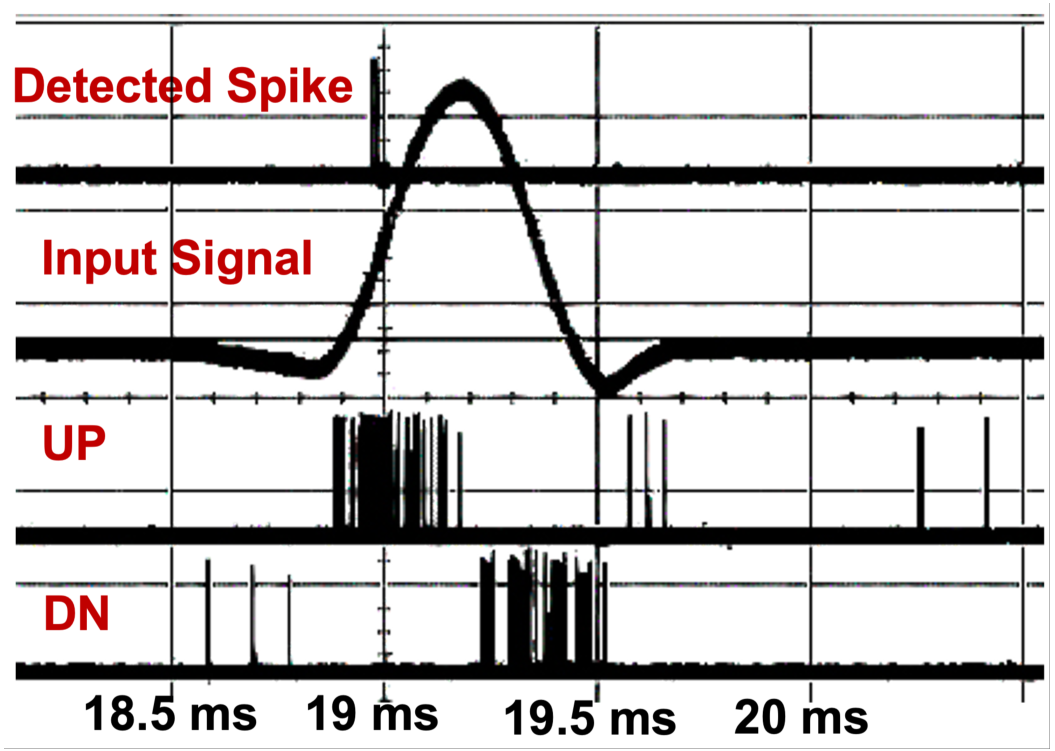
\includegraphics[width=\linewidth]{neuroseed_invivo.png}
    \caption{}
  \end{subfigure}
  \caption[Die CMOS e misura \emph{in vivo} di NeuroSEED]{(a) Die del NeuroSEED e riepilogo prestazioni; (b) Tracciato sperimentale ed eventi \texttt{UP}/\texttt{DN} dell'ASC~\cite{wu2026}.}
  \label{fig:neuroseed_silicio}
\end{figure}

\newpage

\subsection{Rilevamento di crisi epilettiche da iEEG: DYNAP-SE2 (Bartels et al., 2025)}
\label{subsec:dynapse2_app}

Nel paper di Bartels et al.\ (2025)~\cite{bartels2025} il rilevamento delle crisi epilettiche viene testato su segnali registrati sull'uomo, usando il processore neuromorfico mixed-signal DYNAP-SE2. Il chip è CMOS \SI{180}{\nano\meter}, con parti sia analogiche che digitali. Lavora in tempo reale senza un clock globale. Al suo interno ospita 4 core da 256 neuroni analogici AdEx-I\&F ciascuno. Integra sullo stesso die anche il circuito per l'acquisizione e per la codifica ADM già descritto nella sezione~\ref{subsec:vincoli_impiantabili}~\cite{bartels2025}.

Per testare il sistema, gli autori hanno usato i dati di un EEG intracranico (iEEG) del dataset pubblico SWEC-ETHZ. Hanno selezionato 5 pazienti con 2 crisi ciascuno, quindi un totale di 10 crisi. I segnali digitali del dataset sono stati convertiti in forma analogica con un DAC esterno e inviati all'AFE integrato, dove il circuito ADM li trasforma in sequenze di spike~\cite{bartels2025}.

Dato che i circuiti analogici in sottosoglia di DYNAP-SE2 hanno un mismatch piuttosto alto (tra il 20\% e il 30\% sui parametri di polarizzazione) e pesi a bassa precisione, gli autori costruiscono una rete molto semplice, formata da soli due strati di neuroni in cascata con pesi fissi. Il funzionamento si basa sui tempi di risposta delle sinapsi e su come i neuroni sono collegati tra loro. Il primo strato, chiamato strato di traduzione, riceve gli spike dall'ADM e usa tre tipi di neuroni (eccitatori ricorrenti R-E, inibitori ricorrenti R-I e inibitori rapidi FF-I) per bloccare i segnali troppo lenti o troppo veloci e lascia passare solo le frequenze tra \SI{200}{\hertz} e \SI{600}{\hertz}. Il secondo strato, chiamato NLNG (Non-Local Non-Global), collega tra di loro i neuroni usando sinapsi a peso costante. Quando più canali vicini si attivano insieme durante una crisi, i neuroni di quella zona iniziano a sparare molto più velocemente e formano gruppi sincronizzati, come si vede in figura~\ref{fig:dynapse2_sync}~\cite{bartels2025}.

\begin{figure}[tb]
  \centering
  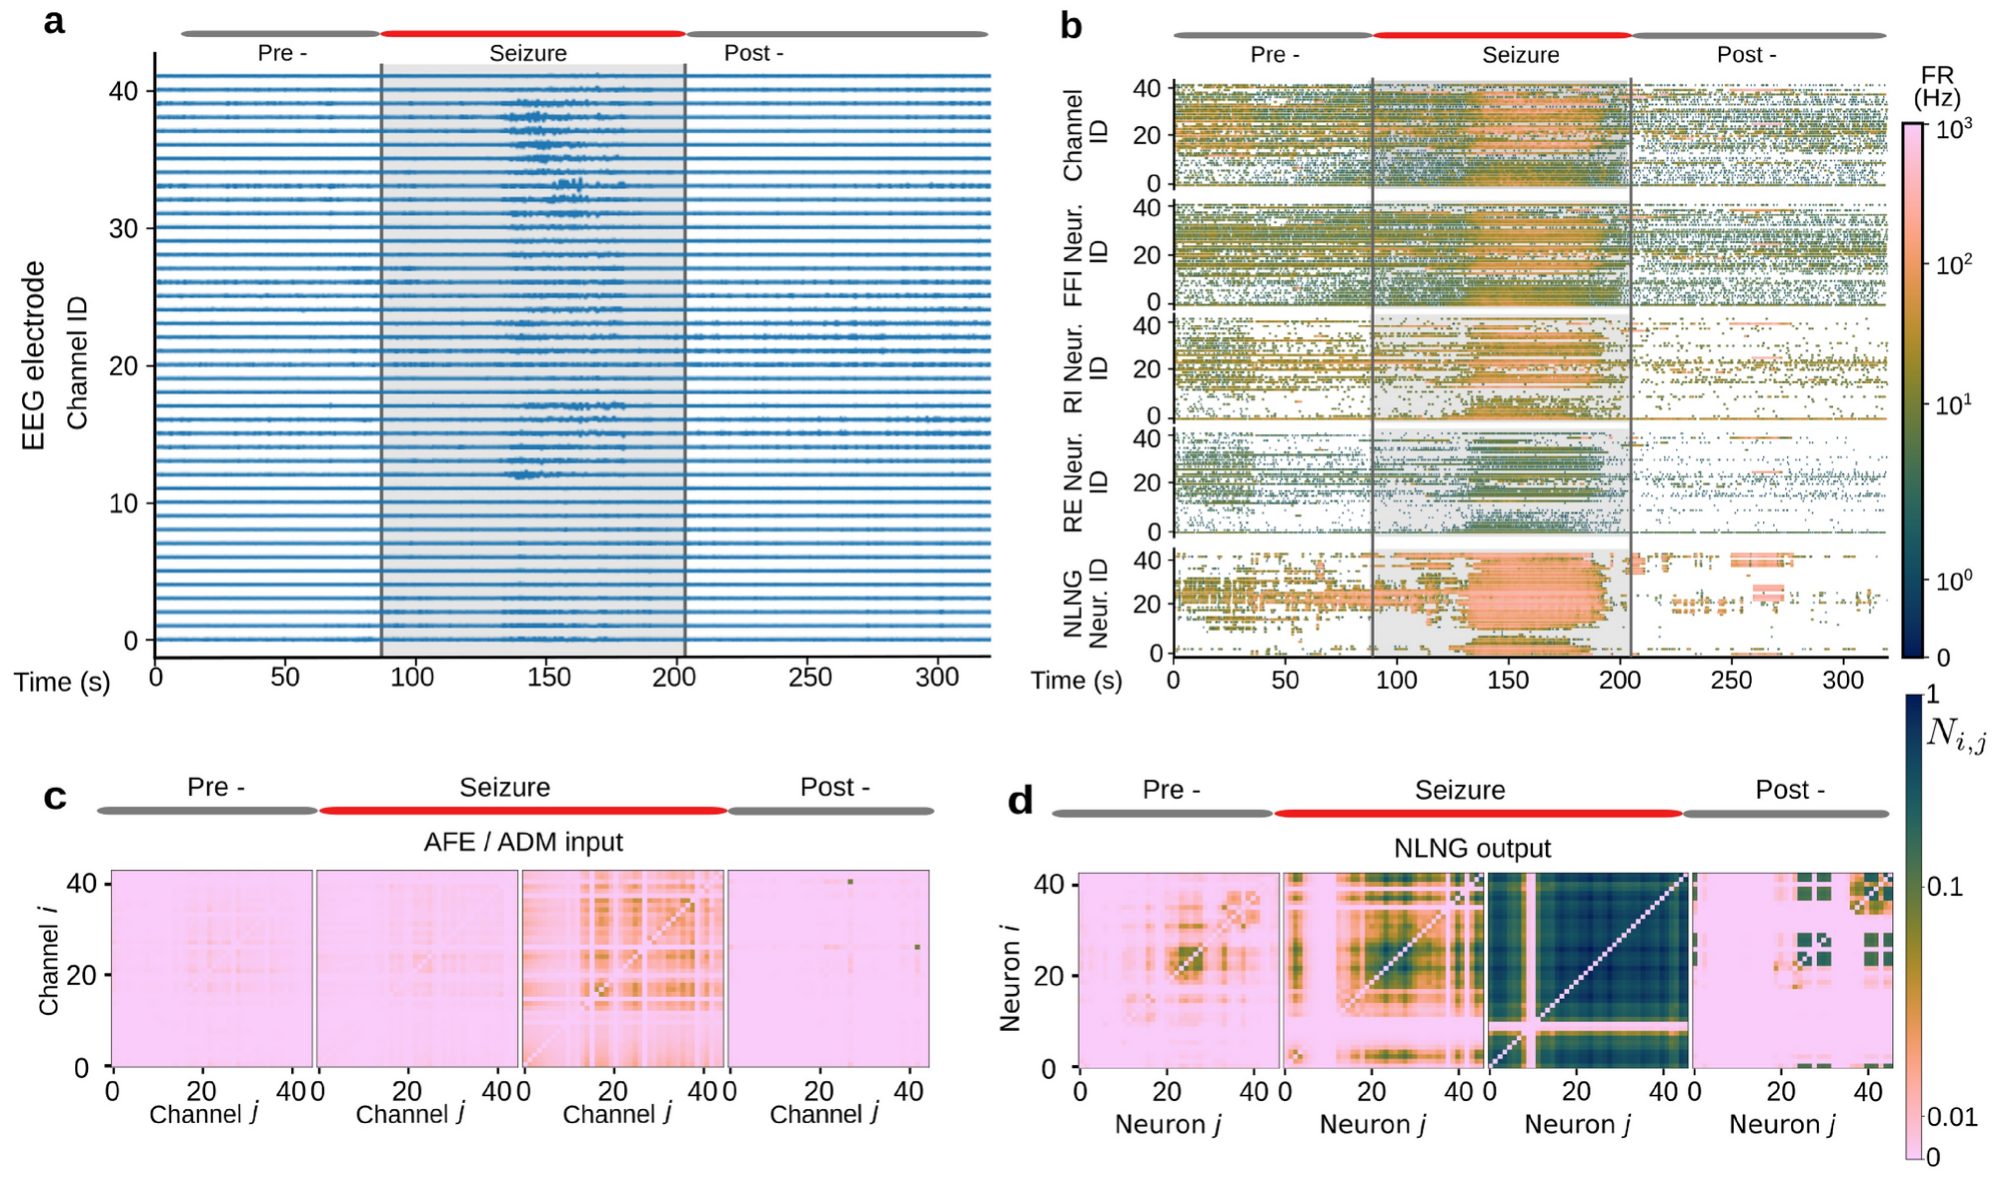
\includegraphics[width=0.96\textwidth]{dynapse2_sync.png}
  \caption[Rilevamento di crisi epilettiche su iEEG umano con DYNAP-SE2]{Elaborazione di 42 canali iEEG (Paziente 1, Crisi 1 del dataset SWEC-ETHZ) su DYNAP-SE2~\cite{bartels2025}: (a) tracciati iEEG con il periodo di crisi evidenziato; (b) sequenze di spike dall'ADM fino allo strato NLNG; (c--d) matrici di sincronizzazione tra canali in ingresso (AFE/ADM) e in uscita (NLNG) prima, durante e dopo la crisi.}
  \label{fig:dynapse2_sync}
\end{figure}

Quindi dallo strato NLNG escono degli spike. Per capire se questi spike sono effettivamente riconducibili ad una crisi, gli autori usano fuori dal chip un classificatore lineare (Linear SVM). Gli spike in uscita vengono divisi in finestre da \SI{1}{\second} e si calcola la frequenza di sparo dei neuroni in ogni finestra. In media sui 5 pazienti si ottiene un'accuratezza del 78,35\% (percentuale totale di finestre classificate correttamente), una sensibilità del 66,71\% (crisi riconosciute), una specificità dell'85,54\% (periodi senza crisi riconosciuti correttamente) e un'AUC dell'80,91\% (indice che riassume il compromesso tra sensibilità e falsi positivi). Gli autori hanno poi confrontato questo risultato dando al classificatore direttamente gli spike dell'ADM senza passare dalla SNN: la rete migliora soprattutto il riconoscimento delle crisi (la sensibilità sale dal 58,56\% al 66,71\%), mentre l'ADM da solo ha una specificità leggermente più alta (89,55\%), cioè riconosce un po' meglio i momenti senza crisi~\cite{bartels2025}.

Per quanto riguarda i consumi, la potenza media stimata a \SI{1{,}8}{\volt} è di circa \SI{150}{\micro\watt}, pari a \SI{2{,}8}{\micro\watt} per canale\cite{bartels2025}.

\subsection{Rilevamento di crisi epilettiche da EEG di scalpo: Xylo (Li et al., 2024)}
\label{subsec:xylo_app}

Nel paper di Li et al.\ (2024)~\cite{li2024} si ua il processore neuromorfico Xylo per riconoscere le crisi epilettiche in tempo reale a partire da registrazioni di EEG di scalpo, cioè acquisite in modo non invasivo con elettrodi sulla testa. Xylo è un processore SNN interamente digitale in tecnologia CMOS \SI{28}{\nano\meter}, occupa \SI{6{,}5}{\milli\meter\squared} e dispone di \SI{124}{\kilo\byte} di memoria SRAM. Può gestire fino a 1000 neuroni LIF digitali (più 8 neuroni di uscita) con pesi a 8 bit. La rete viene prima addestrata via software fuori dal chip e poi i suoi parametri vengono caricati su Xylo~\cite{li2024}.

Gli autori hanno testato il sistema su due dataset pubblici di EEG di scalpo. Prima di arrivare al chip, è stato fatto del filtraggio via software per togliere artefatti come battito cardiaco e movimenti muscolari. Il segnale filtrato viene poi convertito in spike con la codifica Delta-Sigma descritta nella sezione~\ref{subsec:vincoli_impiantabili}~\cite{li2024}.

La rete utilizzata si chiama WaveSense ed è una SNN feed-forward formata da più blocchi in cascata che sfruttano sinapsi con diverse costanti di tempo. Richiede solo 2400 pesi, molti meno rispetto alle reti neurali tradizionali confrontate nel paper, che arrivano anche a diversi milioni di parametri. La rete viene addestrata fuori dal chip con l'algoritmo BPTT (Backpropagation Through Time)~\cite{li2024}.

In simulazione software la rete raggiunge un'accuratezza del 93,3\%. Sul chip invece l'accuratezza scende leggermente all'89,87\%. Su segmenti da \SI{5}{\second}, il ritardo mediano di rilevamento misurato su Xylo è di \SI{0{,}5}{\second}. Per quanto riguarda i consumi, il totale è di \SI{375{,}3}{\micro\watt}, molto più basso rispetto alle soluzioni convenzionali su FPGA confrontate nello studio, che consumano tra \SI{159{,}7}{\milli\watt} e \SI{284}{\milli\watt}~\cite{li2024}. 

Anche per questo esempio, molte fasi come il filtraggio e la codifica Delta-Sigma avvengono fuori dal chip. Inoltre, come osservano gli autori del paper, l'accuratezza resta un po' più bassa rispetto a quella delle reti neurali artificiali tradizionali più grandi~\cite{li2024}.

\subsection{Conclusioni sui pro e contro delle SNN}
\label{subsec:risposta_domanda1}


Quindi, perché usare una SNN in un dispositivo biomedicale impiantabile e quali vantaggi offre rispetto all'elaborazione digitale convenzionale?

Il funzionamento a eventi di una SNN si adatta bene alla natura dei segnali biologici, che sono lenti e passano gran parte del tempo in condizioni normali, cioè gli eventi rilevanti sono concentrati solo in alcuni momenti. Una SNN si attiva solo quando il segnale varia in modo significativo. Un sistema digitale convenzionale invece continua a processare ad ogni ciclo di clock, sprecando energia anche quando non sta succedendo nulla~\cite{ronchini2023, bartels2025, wu2026}.

Per quanto riguarda i consumi, come ho analizzato nella sezione~\ref{subsec:vincoli_impiantabili}, nei lunghi periodi di calma, le tecniche di codifica in spike (tipo ADM o ASC) generano pochissimi impulsi e la rete rimane quasi inattiva, evitando i consumi continui di un clock digitale~\cite{bartels2025, wu2026}. Per esempio, nel caso di NET-TEN, la sola parte di elaborazione, cioè una piccola rete analogica in sottosoglia, consuma appena \SI{3{,}50}{\nano\watt} (paragonabili a un singolo neurone biologico)~\cite{ronchini2023}. Con il processore mixed-signal DYNAP-SE2 si stimano circa \SI{150}{\micro\watt} (\SI{2{,}8}{\micro\watt} per canale)~\cite{bartels2025}. E anche un chip SNN interamente digitale come Xylo si ferma a \SI{375{,}3}{\micro\watt} totali, molto al di sotto delle soluzioni convenzionali su FPGA confrontate nel paper, che arrivano a consumare tra \SI{159{,}7}{\milli\watt} e \SI{284}{\milli\watt}~\cite{li2024}.

Per quanto riguarda la latenza, è molto importante affinché un sistema riconosca e risponda ad una crisi in tempo~\cite{ronchini2023}. Rispetto ai sistemi tradizionali che accumulano prima grandi blocchi di segnale in memoria, le SNN elaborano i dati in tempo reale mentre arrivano, sfruttando circuiti con costanti di tempo paragonabili a quelle dei segnali biologici~\cite{ronchini2023, bartels2025, li2024}. NET-TEN risponde in media in \SI{110{,}4}{\milli\second} a una crisi ictale~\cite{ronchini2023}. Xylo rileva le crisi con un ritardo mediano di \SI{0{,}5}{\second} su segmenti da \SI{5}{\second}~\cite{li2024}. Stiamo parlando di tempi decisamente più bassi rispetto ad altre soluzioni convenzionali confrontate nei paper, che arrivano anche a diversi secondi~\cite{ronchini2023}.

Poi c'è la possibilità di elaborare i segnali localmente sul chip, vicino agli elettrodi. Nei dispositivi convenzionali con anche migliaia di canali, trasmettere continuamente via wireless tutti i segnali grezzi consuma troppa energia~\cite{ronchini2023, wu2026}. Grazie all'estrazione direttamente sul chip dei soli eventi utili (come i potenziali d'azione o l'inizio di una crisi), si riduce il volume di dati da inviare all'esterno. In NeuroSEED il trasmettitore wireless consuma in media solo \SI{4{,}6}{\micro\watt} totali (su \SI{63{,}61}{\micro\watt} dell'intero chip a 32 canali)~\cite{wu2026}.

Quindi complessivamente le SNN offrono un vantaggio concreto nei dispositivi impiantabili perché danno bassi consumi, tempi di risposta ridotti ed elaborazione locale. Restano però alcuni limiti emersi nei vari paper. In quasi tutti i prototipi visti, alcune fasi come l'acquisizione, il filtraggio e la codifica in spike avvengono ancora fuori dal chip, quindi i consumi riportati riguardano solo una parte dell'intero sistema. Inoltre c'è il problema del mismatch nei circuiti in sottosoglia (che ad esempio in NET-TEN rende utili solo 4 canali su 10), e l'accuratezza che resta un po' più bassa rispetto alle reti neurali tadizionali più grandi~\cite{ronchini2023, bartels2025, li2024, wu2026}.
